\section{Мета}
Отримання практичних навичок встановлення та
налаштування віртуальних машин.

\section{Хід роботи}
\subsection{Процесс встановлення віртуальної машини}
Конфігурації віртуальної машини:
\begin{itemize}
    \item 512МБ ОЗУ
    \item 20ГБ місця
    \item 1 ядро CPU
\end{itemize}

\begin{figure}[ht!]
    \centering
    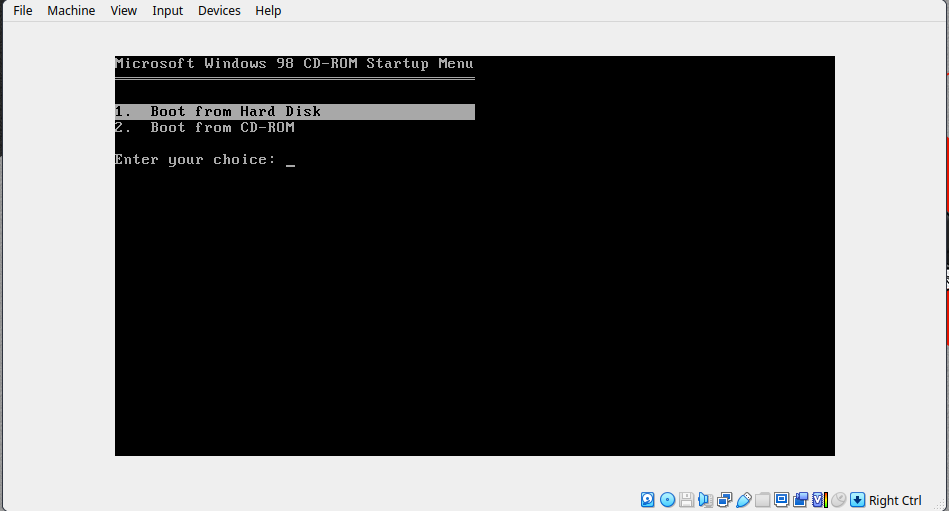
\includegraphics[width=0.7\textwidth]{\assetsDirectory/1.png}
    \caption{Встановлення віртуальної машини з \textbf{Windows98}}
\end{figure}

\newpage
\begin{figure}[ht!]
    \centering
    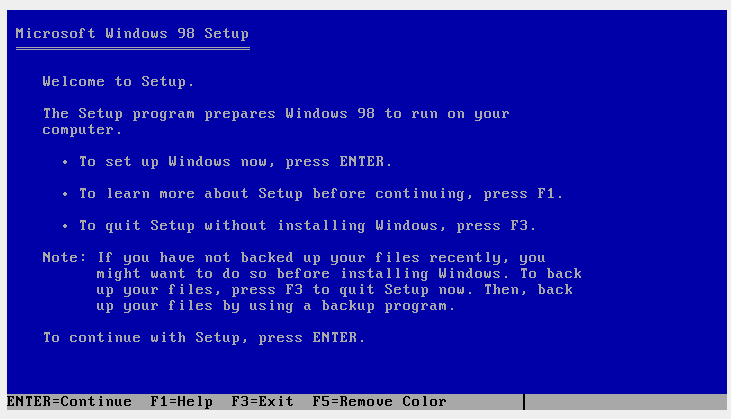
\includegraphics[width=0.7\textwidth]{\assetsDirectory/2.png}
    \caption{Встановлення віртуальної машини з \textbf{Windows98}}
\end{figure}

\begin{figure}[ht!]
    \centering
    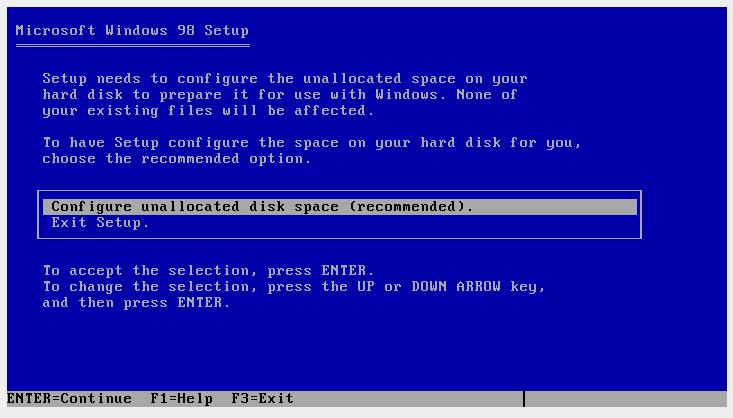
\includegraphics[width=0.7\textwidth]{\assetsDirectory/3.png}
    \caption{Встановлення віртуальної машини з \textbf{Windows98}}
\end{figure}

\begin{figure}[ht!]
    \centering
    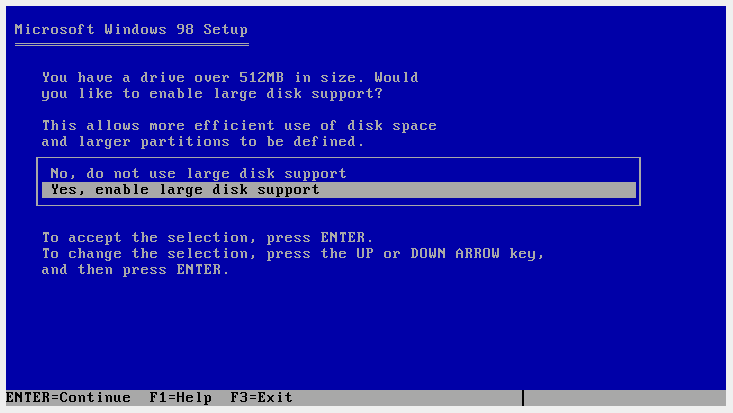
\includegraphics[width=0.7\textwidth]{\assetsDirectory/4.png}
    \caption{Встановлення віртуальної машини з \textbf{Windows98}}
\end{figure}

\begin{figure}[ht!]
    \centering
    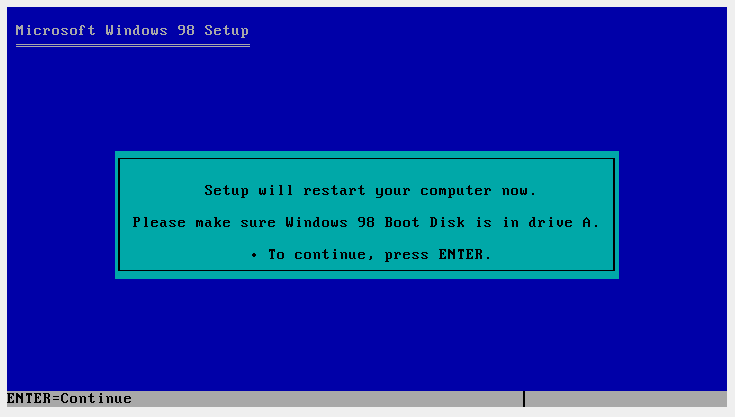
\includegraphics[width=0.7\textwidth]{\assetsDirectory/5.png}
    \caption{Встановлення віртуальної машини з \textbf{Windows98}}
\end{figure}

\begin{figure}[ht!]
    \centering
    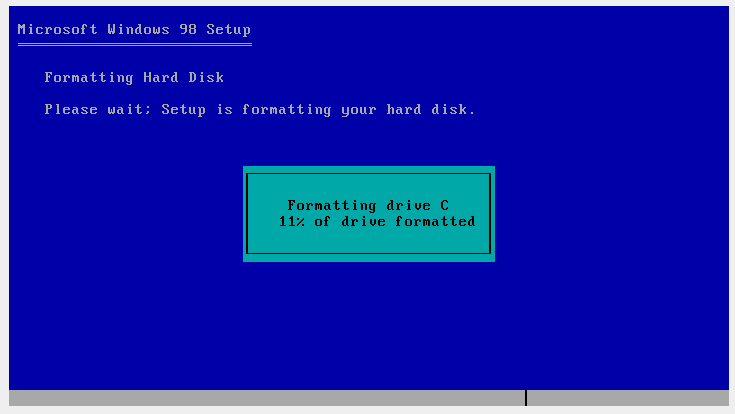
\includegraphics[width=0.7\textwidth]{\assetsDirectory/6.png}
    \caption{Встановлення віртуальної машини з \textbf{Windows98}}
\end{figure}

\begin{figure}[ht!]
    \centering
    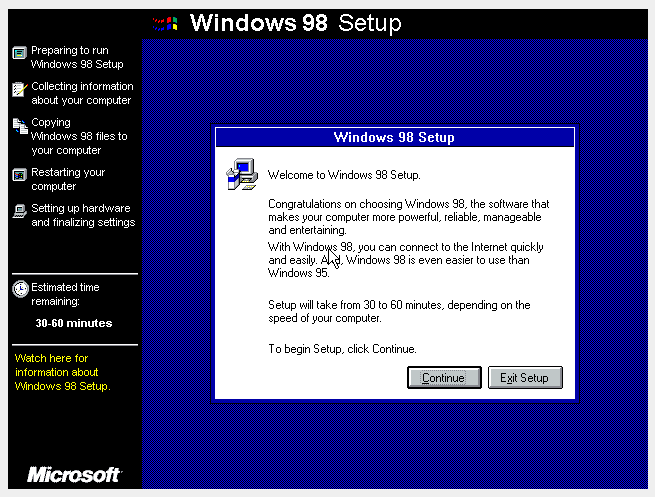
\includegraphics[width=0.7\textwidth]{\assetsDirectory/7.png}
    \caption{Встановлення віртуальної машини з \textbf{Windows98}}
\end{figure}

\begin{figure}[ht!]
    \centering
    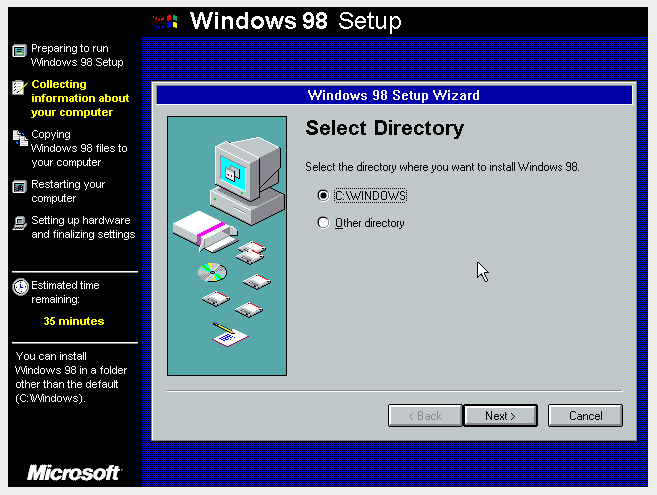
\includegraphics[width=0.7\textwidth]{\assetsDirectory/8.png}
    \caption{Встановлення віртуальної машини з \textbf{Windows98}}
\end{figure}

\begin{figure}[ht!]
    \centering
    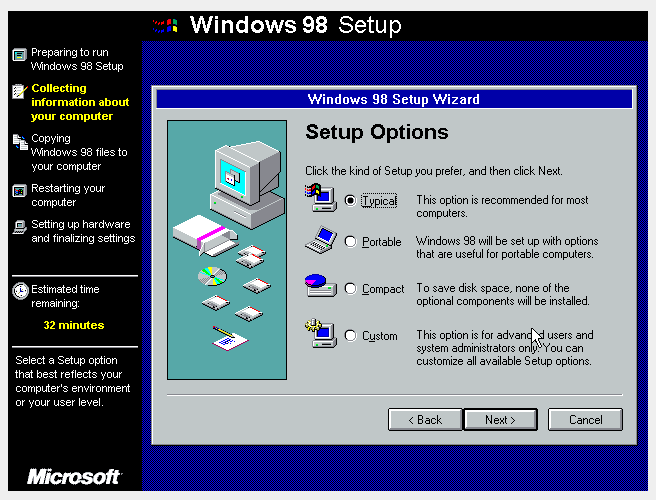
\includegraphics[width=0.7\textwidth]{\assetsDirectory/9.png}
    \caption{Встановлення віртуальної машини з \textbf{Windows98}}
\end{figure}

\begin{figure}[ht!]
    \centering
    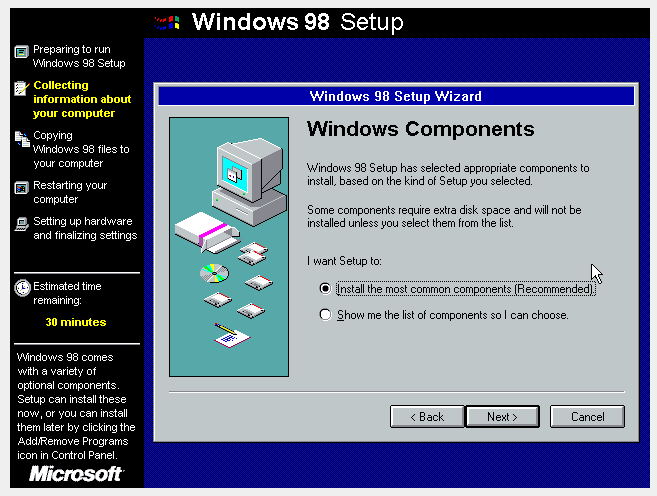
\includegraphics[width=0.7\textwidth]{\assetsDirectory/10.png}
    \caption{Встановлення віртуальної машини з \textbf{Windows98}}
\end{figure}

\begin{figure}[ht!]
    \centering
    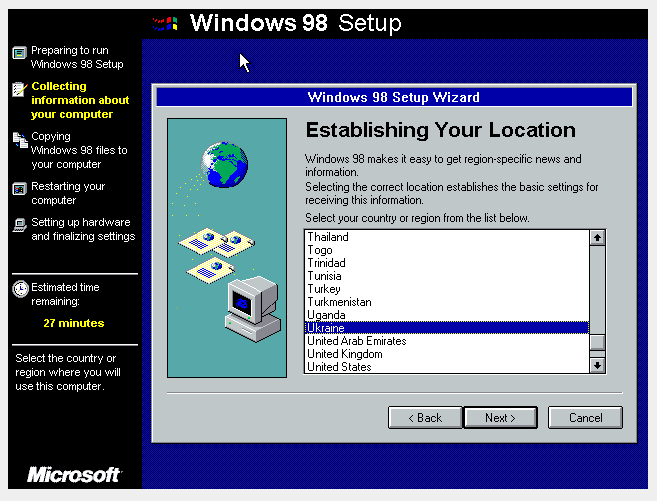
\includegraphics[width=0.7\textwidth]{\assetsDirectory/11.png}
    \caption{Встановлення віртуальної машини з \textbf{Windows98}}
\end{figure}

\begin{figure}[ht!]
    \centering
    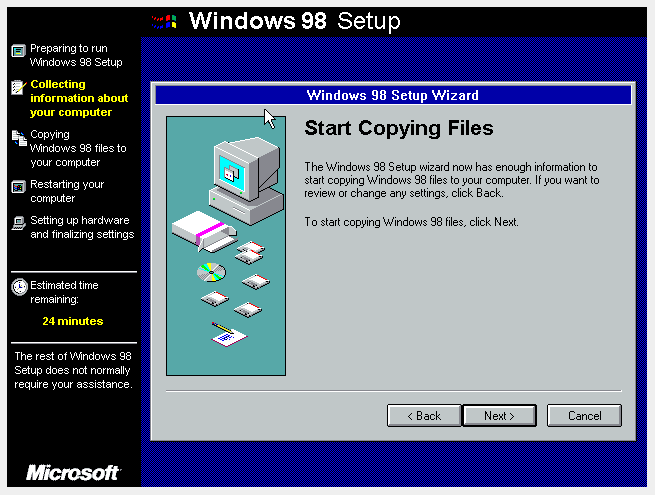
\includegraphics[width=0.7\textwidth]{\assetsDirectory/12.png}
    \caption{Встановлення віртуальної машини з \textbf{Windows98}}
\end{figure}

\begin{figure}[ht!]
    \centering
    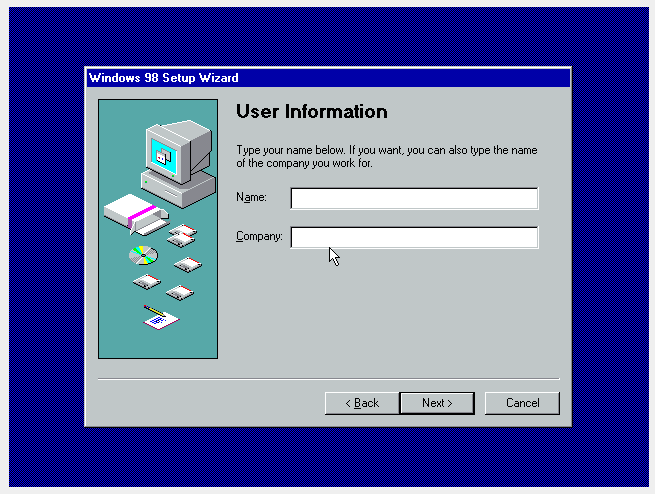
\includegraphics[width=0.7\textwidth]{\assetsDirectory/14.png}
    \caption{Встановлення віртуальної машини з \textbf{Windows98}}
\end{figure}

\begin{figure}[ht!]
    \centering
    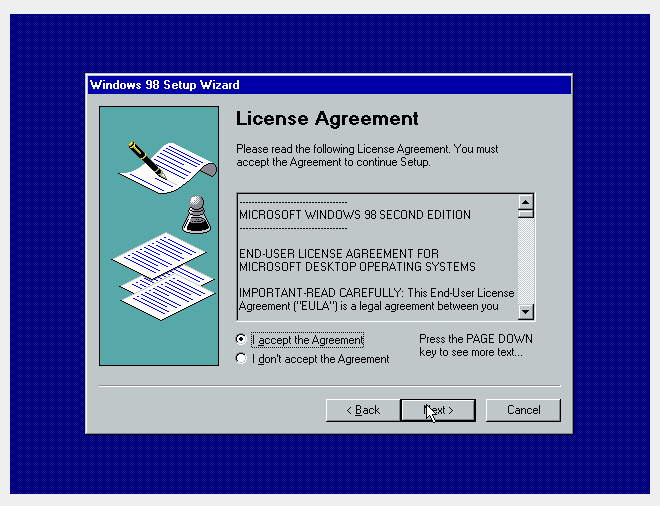
\includegraphics[width=0.7\textwidth]{\assetsDirectory/15.png}
    \caption{Встановлення віртуальної машини з \textbf{Windows98}}
\end{figure}

\begin{figure}[ht!]
    \centering
    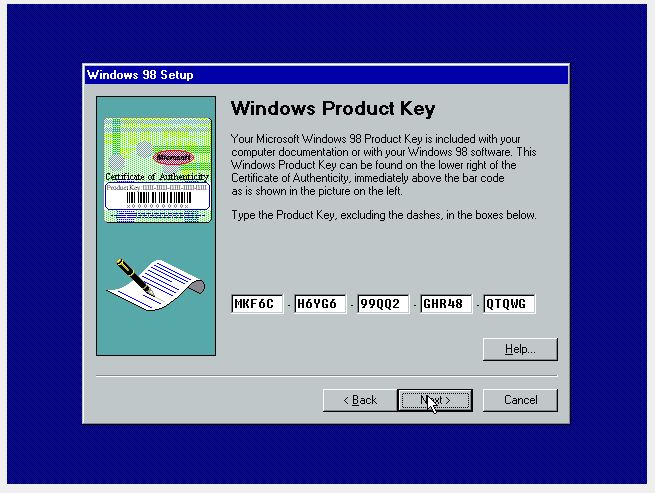
\includegraphics[width=0.7\textwidth]{\assetsDirectory/16.png}
    \caption{Встановлення віртуальної машини з \textbf{Windows98}}
\end{figure}

\begin{figure}[ht!]
    \centering
    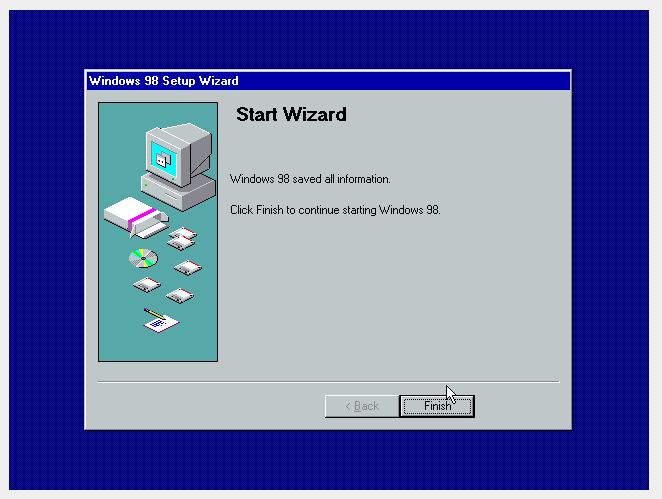
\includegraphics[width=0.7\textwidth]{\assetsDirectory/17.png}
    \caption{Встановлення віртуальної машини з \textbf{Windows98}}
\end{figure}

\begin{figure}[ht!]
    \centering
    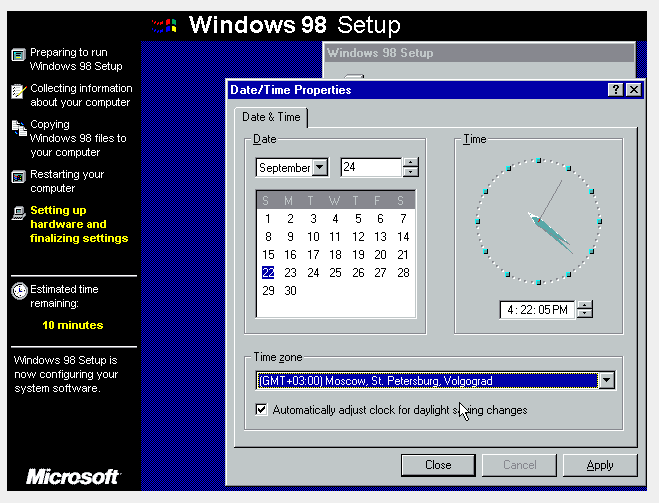
\includegraphics[width=0.7\textwidth]{\assetsDirectory/18.png}
    \caption{Встановлення віртуальної машини з \textbf{Windows98}}
\end{figure}

\clearpage

\subsection{Встановлення серди розробки \textbf{BorlandC}}
\begin{figure}[ht!]
    \centering
    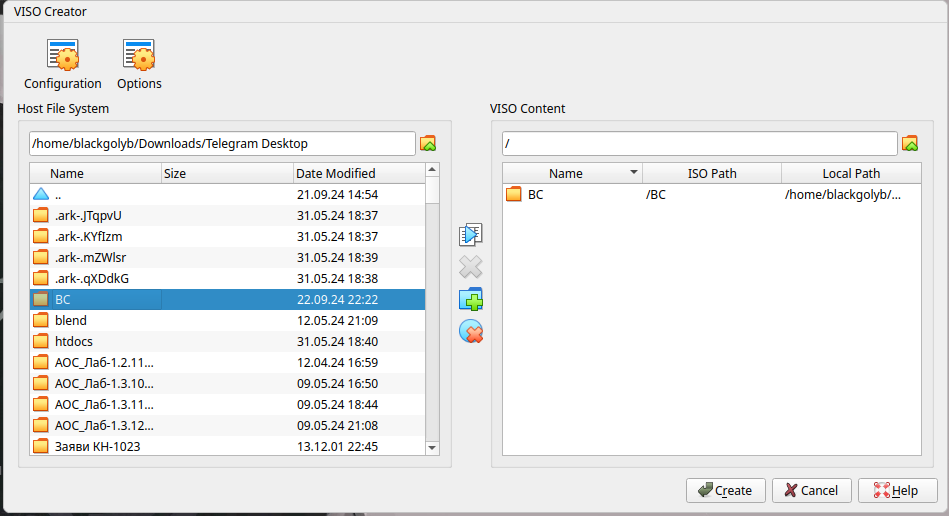
\includegraphics[width=0.7\textwidth]{\assetsDirectory/bc_1.png}
    \caption{Переносимо \textbf{BorlandC} на віртуальну машину}
\end{figure}

\begin{figure}[ht!]
    \centering
    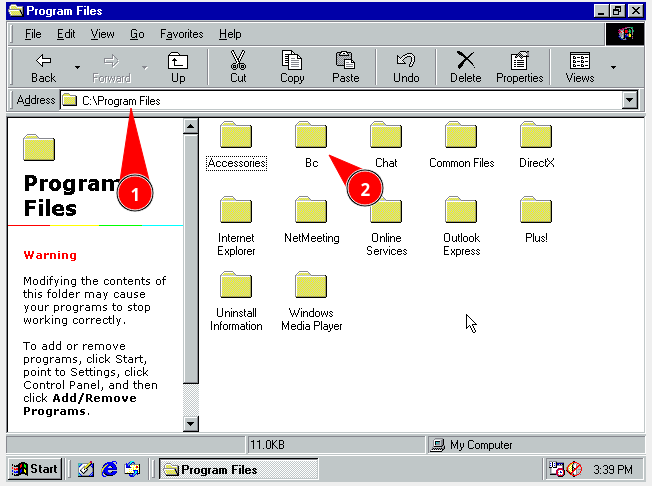
\includegraphics[width=0.7\textwidth]{\assetsDirectory/bc_2.png}
    \caption{Переносимо \textbf{BorlandC} на віртуальну машину}
\end{figure}

\begin{figure}[ht!]
    \centering
    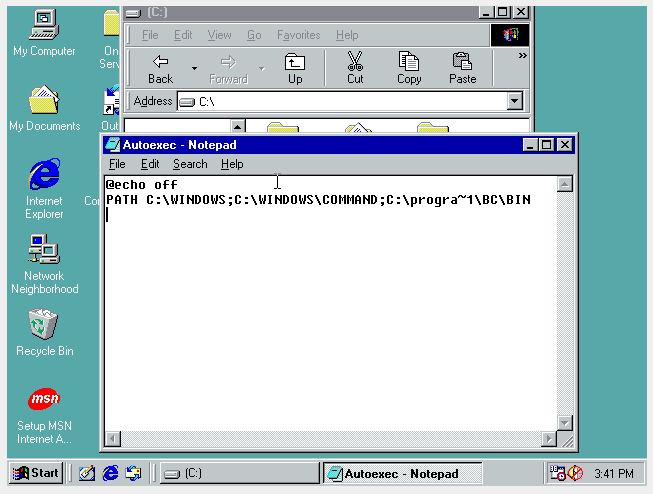
\includegraphics[width=0.7\textwidth]{\assetsDirectory/bc_3.png}
    \caption{Додаємо \textbf{BorlandC} у PATH}
\end{figure}

\begin{figure}[ht!]
    \centering
    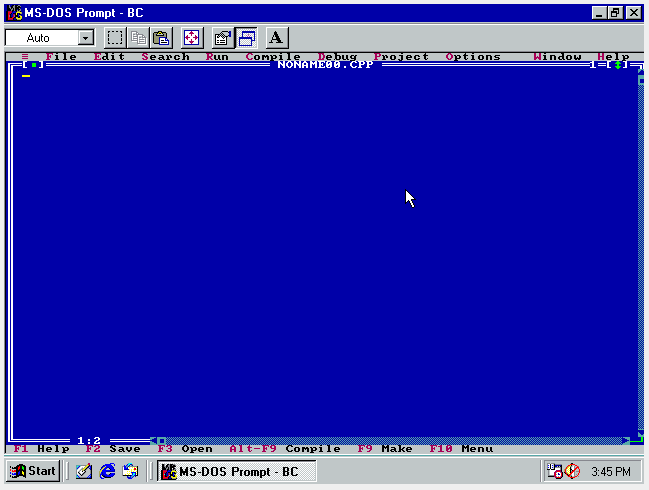
\includegraphics[width=0.7\textwidth]{\assetsDirectory/bc_4.png}
    \caption{Запуск \textbf{BorlandC}}
\end{figure}

\begin{figure}[ht!]
    \centering
    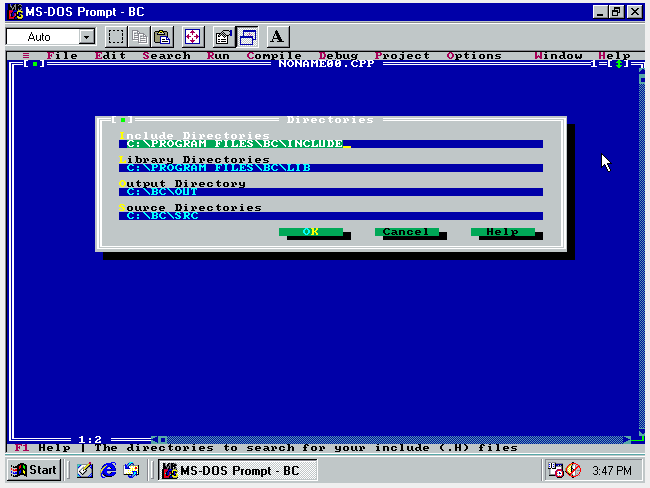
\includegraphics[width=0.7\textwidth]{\assetsDirectory/bc_5.png}
    \caption{Налаштування директорій для \textbf{BorlandC}}
\end{figure}

\clearpage
\section{Висновки}
В ході виконання практичної робити було отримано навички використання віртуальних машин та встановлено
\textbf{Windows98}. Також було встановлено та налаштовано середу розробки \textbf{BorlandC}.